\section{Diseño del sistema}
Cuando se empieza con el desarrollo de un proyecto lo primero por hacer es el análisis, en él se puede hacer uso de una herramienta llamada “UML” que no es otra cosa más que un estándar para la creación de esquemas, diagramas y documentación que describan el funcionamiento y comportamiento del sistema por desarrollar.
\subsection{Del análsis al diseño}
Para que nuestro sistema se puede entender y desarrollar correctamente se hace uso de 8 tipos de diagramas, entre los cuales están de estados, actividades, secuencia, colaboración, casos de uso, componentes, distribución y procesos.
\subsection{Diagramas UML}
UML es una poderosa herramienta con la cual es posible establecer la serie de requerimientos y estructuras necesarias para plasmar un sistema de software previo al proceso intensivo de escribir código, en pocas palabras, así como en la construcción de un edificio se realizan planos previos a su construcción, en Software se deben realizar diseños del sistema antes de empezar a programar, de esta manera se evitan errores lógicos para obtener un sistema de buena calidad.
\subsubsection{Diagramas de Casos de uso y estados}


\begin{figure}[htb]
\begin{center}
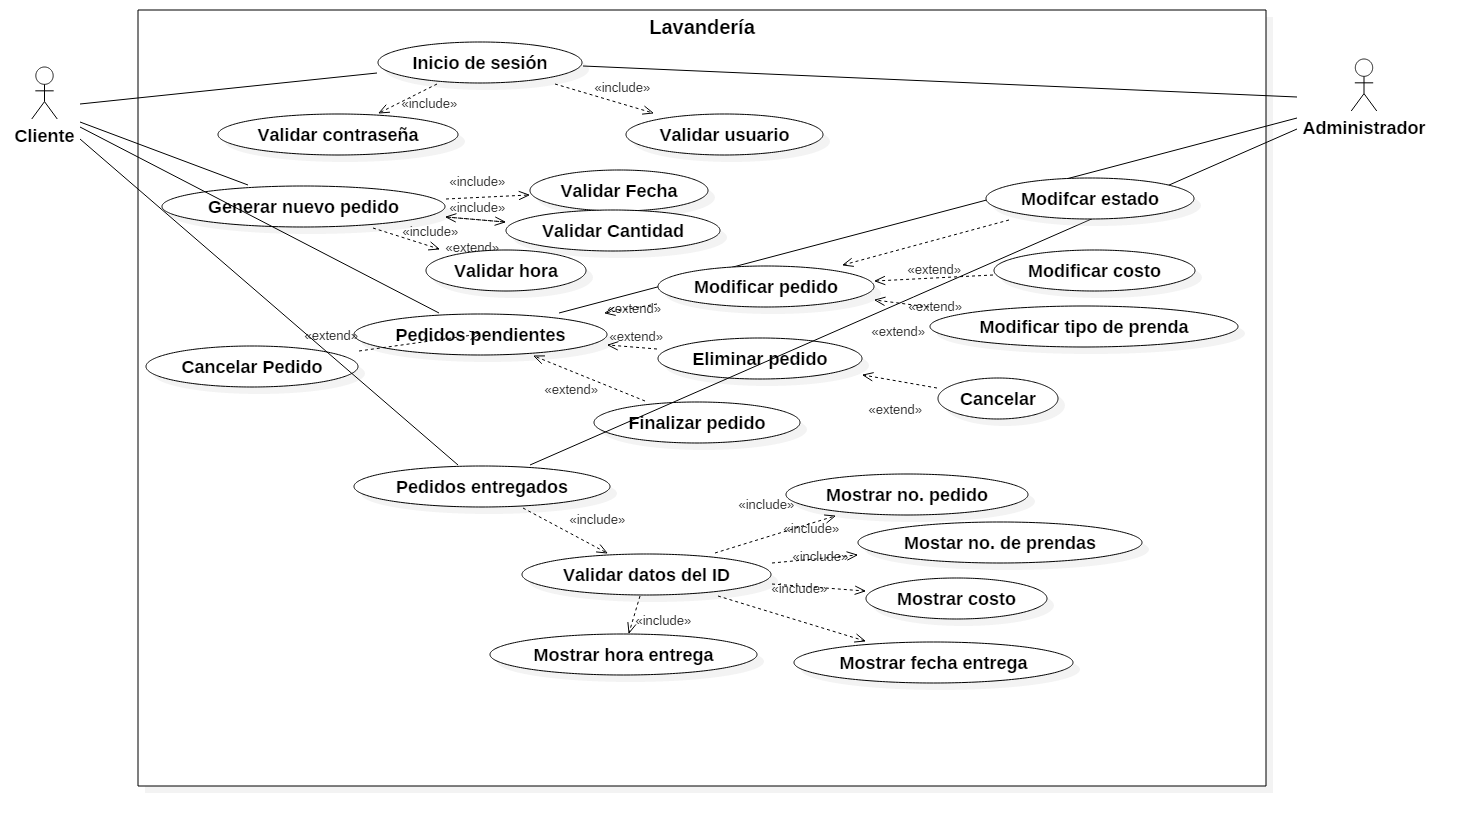
\includegraphics[width=18cm]{./imagenes/diagramas/CU_Lavanderia.png}
\end{center}
\caption{CU general del sistema}
\end{figure}


\begin{figure}[htb]
\begin{center}
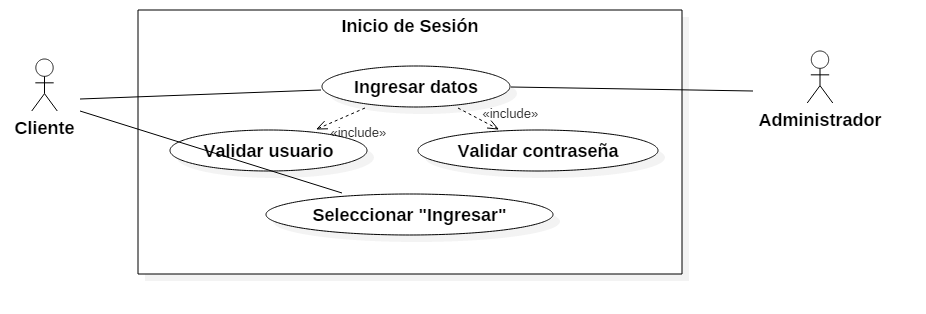
\includegraphics[width=15cm]{./imagenes/diagramas/CU_IniciarSesion.png}
\end{center}
\caption{Inicio de sesión}
\end{figure}


\begin{figure}[htb]
\begin{center}
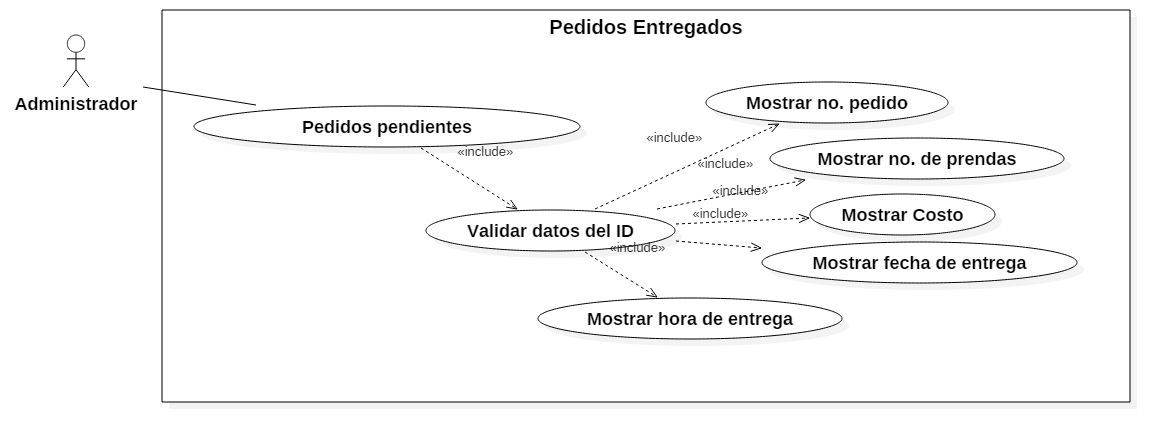
\includegraphics[width=15cm]{./imagenes/diagramas/CU_PedidosEntregados(Admin).png}
\end{center}
\caption{CU de Pedidos entregados del Administrador}
\end{figure}


\begin{figure}[htb]
\begin{center}
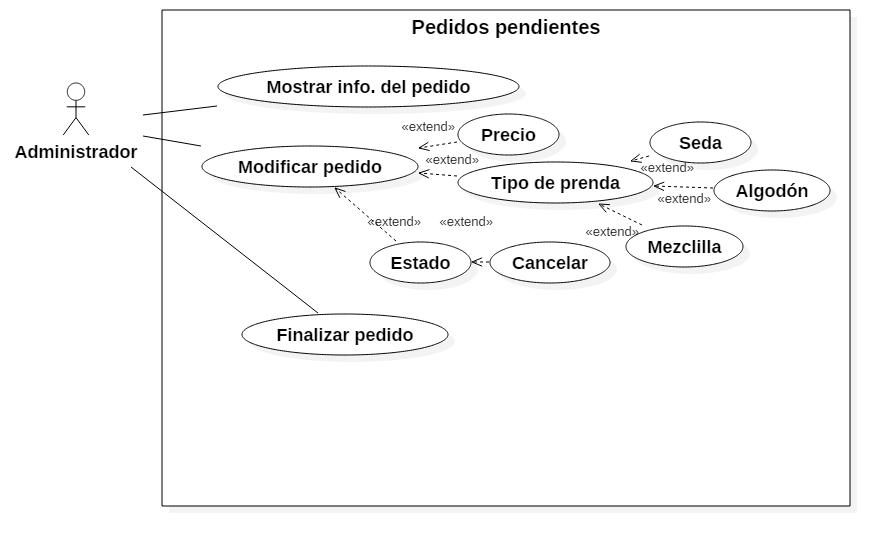
\includegraphics[width=15cm]{./imagenes/diagramas/CU_PedidosPendientes(Admin).png}
\end{center}
\caption{CU de pedidos pendientes del Administrador}
\end{figure}


\begin{figure}[htb]
\begin{center}
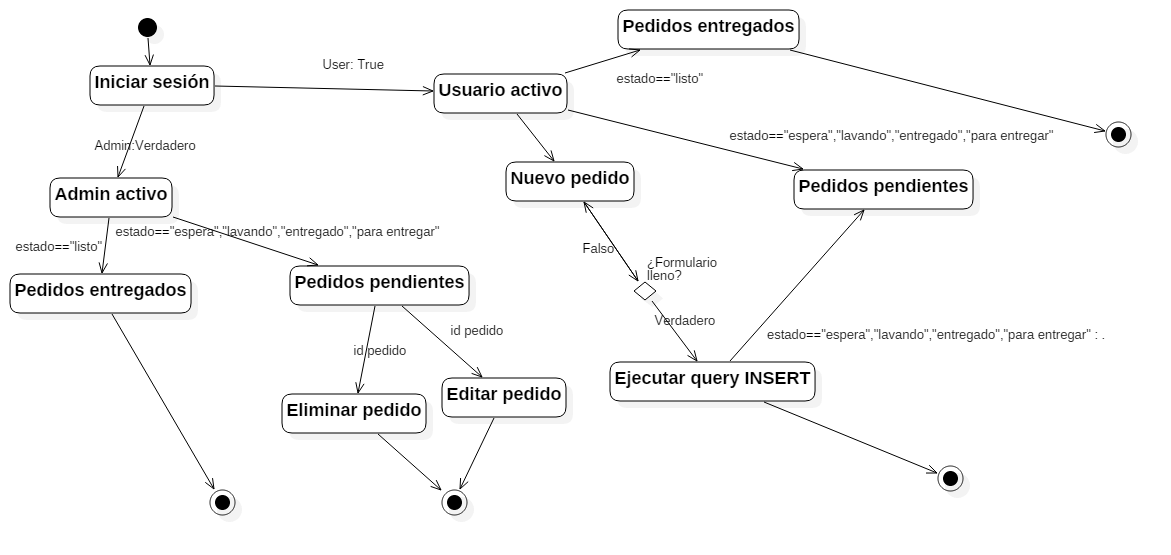
\includegraphics[width=18cm]{./imagenes/diagramas/Estado_lavanderia.png}
\end{center}
\caption{Diagrama de estados del sistema}
\end{figure}


\begin{figure}[htb]
\begin{center}
\includegraphics[width=6cm]{./imagenes/diagramas/Estados_lavanderia2.png}
\end{center}
\caption{Diagrama de estados de un nuevo pedido}
\end{figure}


\newpage

\subsubsection{Diagramas de clases y objetos}




\subsubsection{Diagramas de procesos y actividades}


\begin{figure}[htb]
\begin{center}
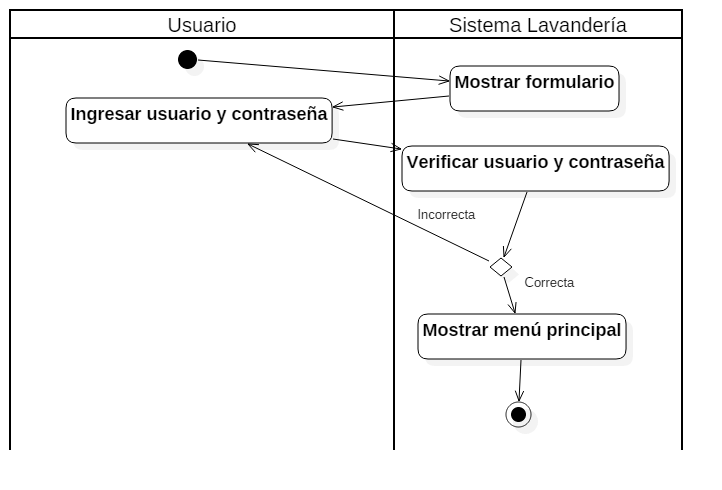
\includegraphics[width=10cm]{./imagenes/diagramas/Actividades_Lavanderia_InicioSesion.png}
\end{center}
\caption{Diagrama de actividades de inicio de sesion}
\end{figure}

\begin{figure}[htb]
\begin{center}
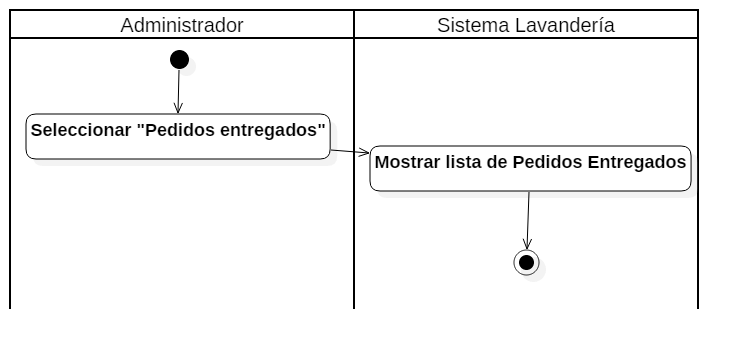
\includegraphics[width=10cm]{./imagenes/diagramas/Actividades_Lavanderia_PedidosEntregados.png}
\end{center}
\caption{Diagrama de actividades de Pedidos entregados}
\end{figure}

\begin{figure}[htb]
\begin{center}
\includegraphics[width=10cm]{./imagenes/diagramas/Actividades_Lavanderia_PedidosPendientes.png}
\end{center}
\caption{Diagrama de estados de pedidos pendientes}
\end{figure}

\newpage


\subsubsection{Diagramas de secuencia y colaboracion}

\begin{figure}[htb]
\begin{center}
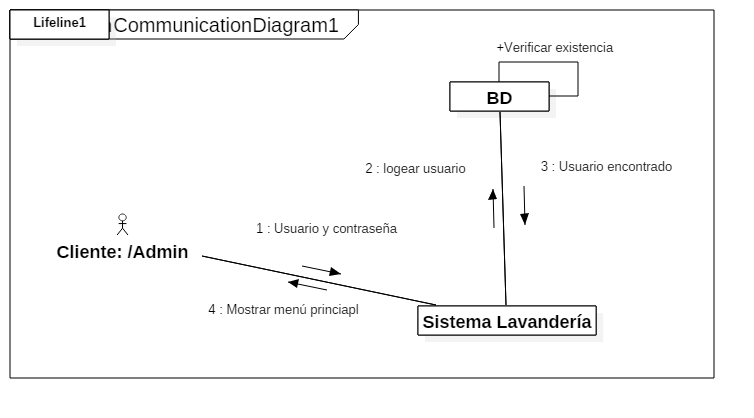
\includegraphics[width=10cm]{./imagenes/diagramas/Colaboracion_IniciarSesion.png}
\end{center}
\caption{Diagrama de Colaboración:Inicio de sesion}
\end{figure}


\begin{figure}[htb]
\begin{center}
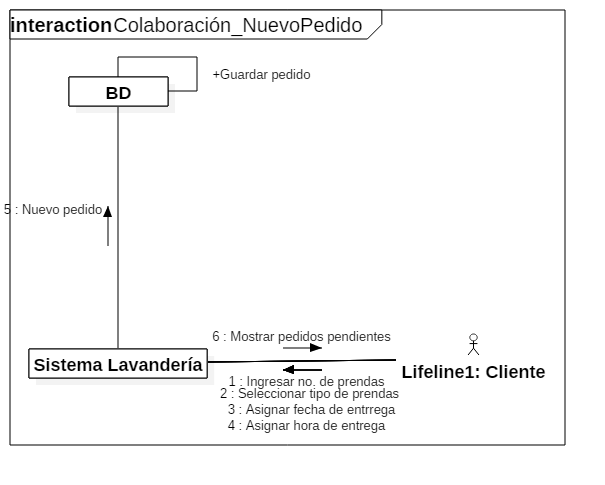
\includegraphics[width=10cm]{./imagenes/diagramas/Colaboracion_NuevoPedido.png}
\end{center}
\caption{Diagrama de Colaboracíon:Nuevo pedido}
\end{figure}


\begin{figure}[htb]
\begin{center}
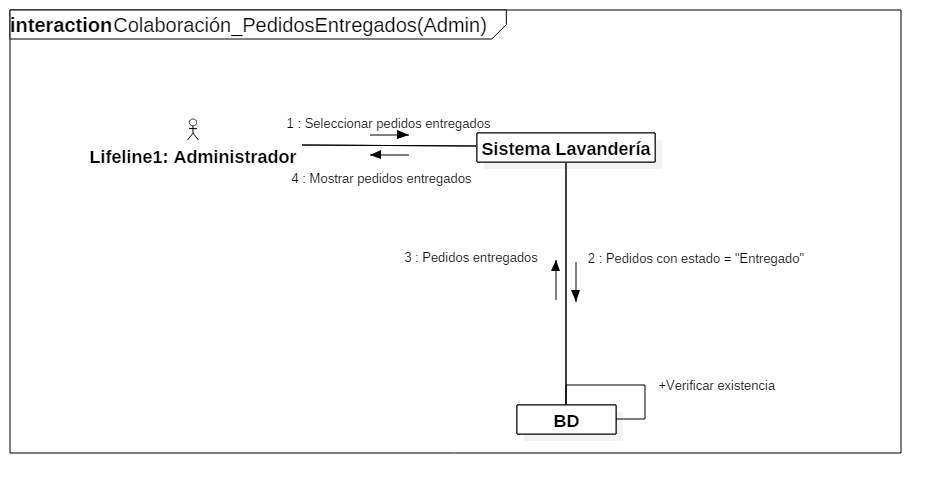
\includegraphics[width=10cm]{./imagenes/diagramas/Colaboracion_PedidosEntregados(Admin).png}
\end{center}
\caption{Diagrama de Colaboración: Pedidos entregados -Admin}
\end{figure}


\begin{figure}[htb]
\begin{center}
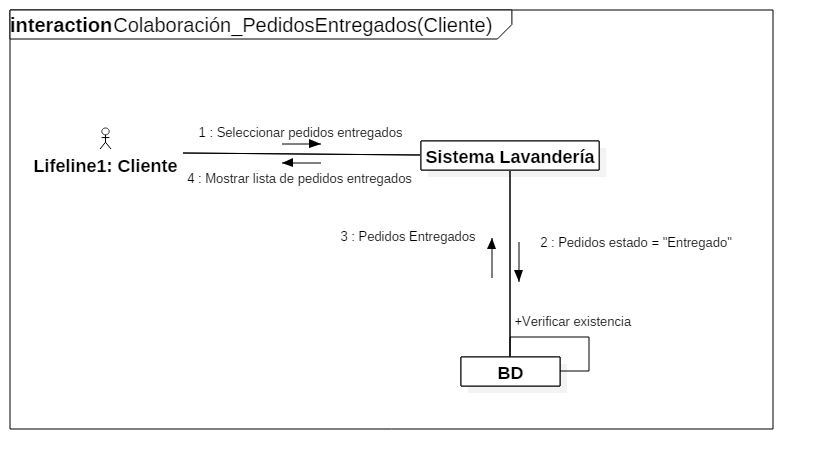
\includegraphics[width=10cm]{./imagenes/diagramas/Colaboracion_PedidosEntregados(Cliente).png}
\end{center}
\caption{Diagrama de Colaboración: Pedidos entregados -Cliente}
\end{figure}


\begin{figure}[htb]
\begin{center}
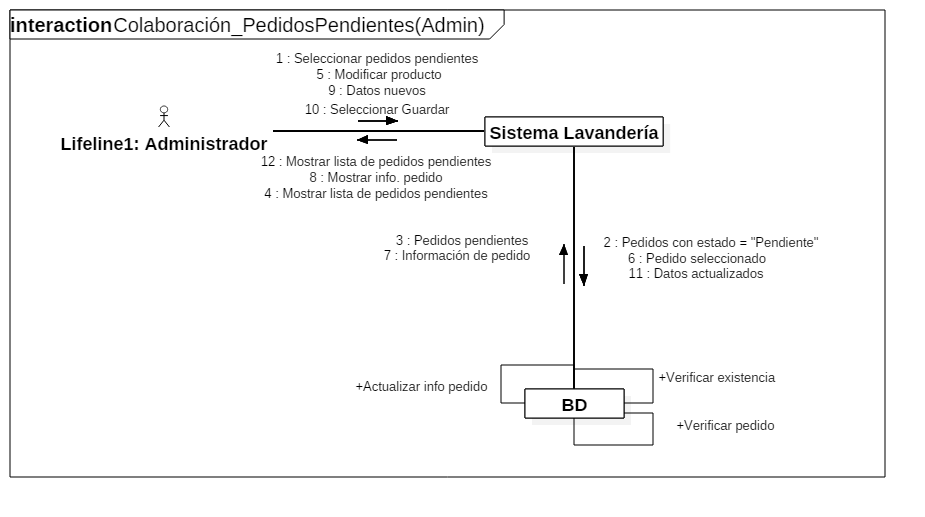
\includegraphics[width=10cm]{./imagenes/diagramas/Colaboracion_PedidosPendientes(Admin).png}
\end{center}
\caption{Diagrama de Colaboración: Pedidos Pendientes -Admin }
\end{figure}


\begin{figure}[htb]
\begin{center}
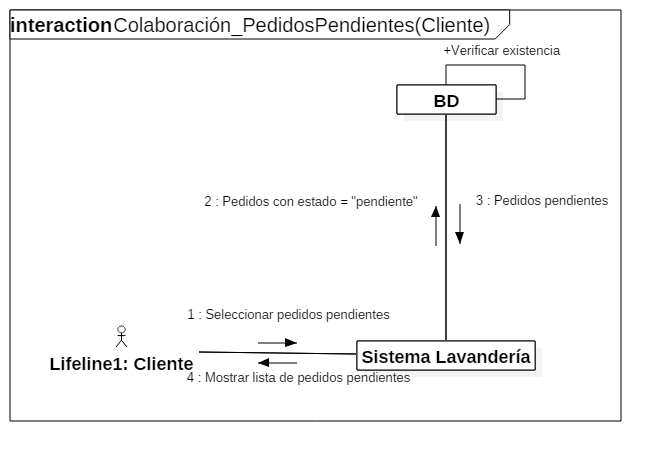
\includegraphics[width=10cm]{./imagenes/diagramas/Colaboracion_PedidosPendientes(Cliente).png}
\end{center}
\caption{Diagrama de Colaboración: Pedidos Pendientes -Cliente}
\end{figure}



\begin{figure}[htb]
\begin{center}
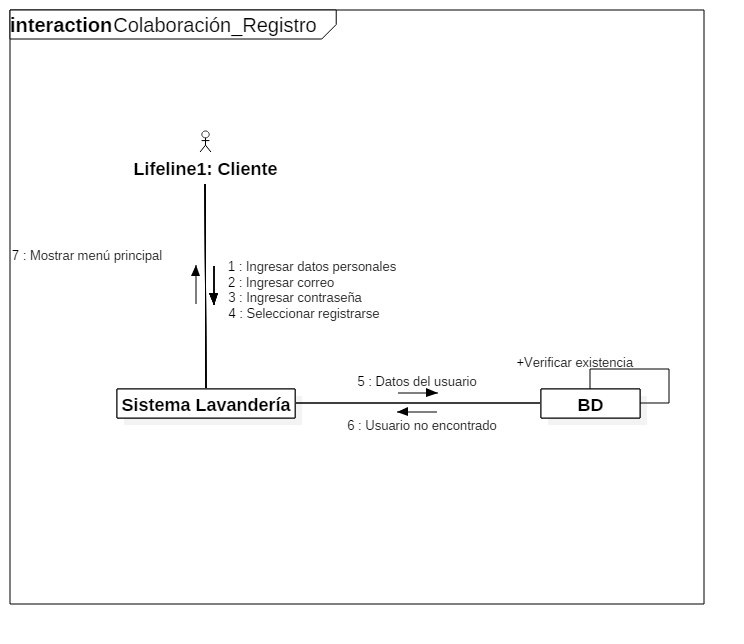
\includegraphics[width=10cm]{./imagenes/diagramas/Colaboracion_Registro.png}
\end{center}
\caption{Diagrama de Colaboración: Registro}
\end{figure}



%Diagramas de secuencia


\begin{figure}[htb]
\begin{center}
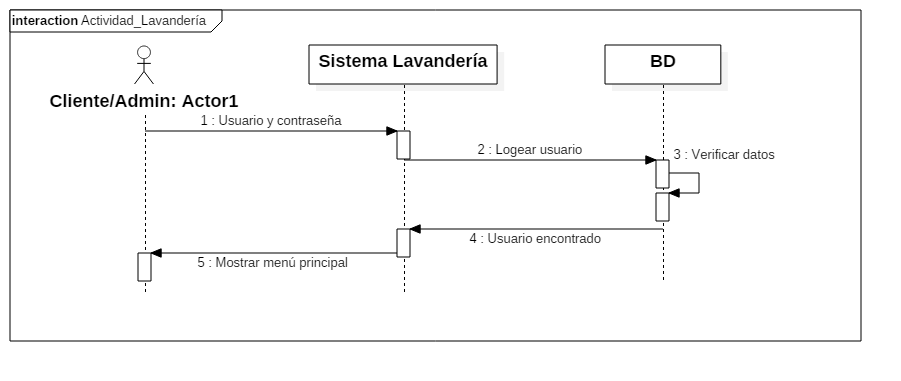
\includegraphics[width=10cm]{./imagenes/diagramas/Secuencia_InicioSesion.png}
\end{center}
\caption{Diagrama de Secuencia:Inicio de sesion}
\end{figure}


\begin{figure}[htb]
\begin{center}
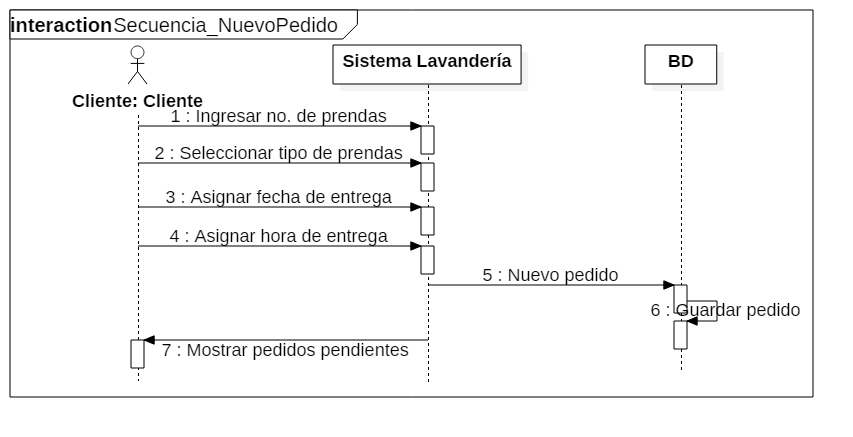
\includegraphics[width=10cm]{./imagenes/diagramas/Secuencia_NuevoPedido.png}
\end{center}
\caption{Diagrama de Secuencia:Nuevo pedido}
\end{figure}


\begin{figure}[htb]
\begin{center}
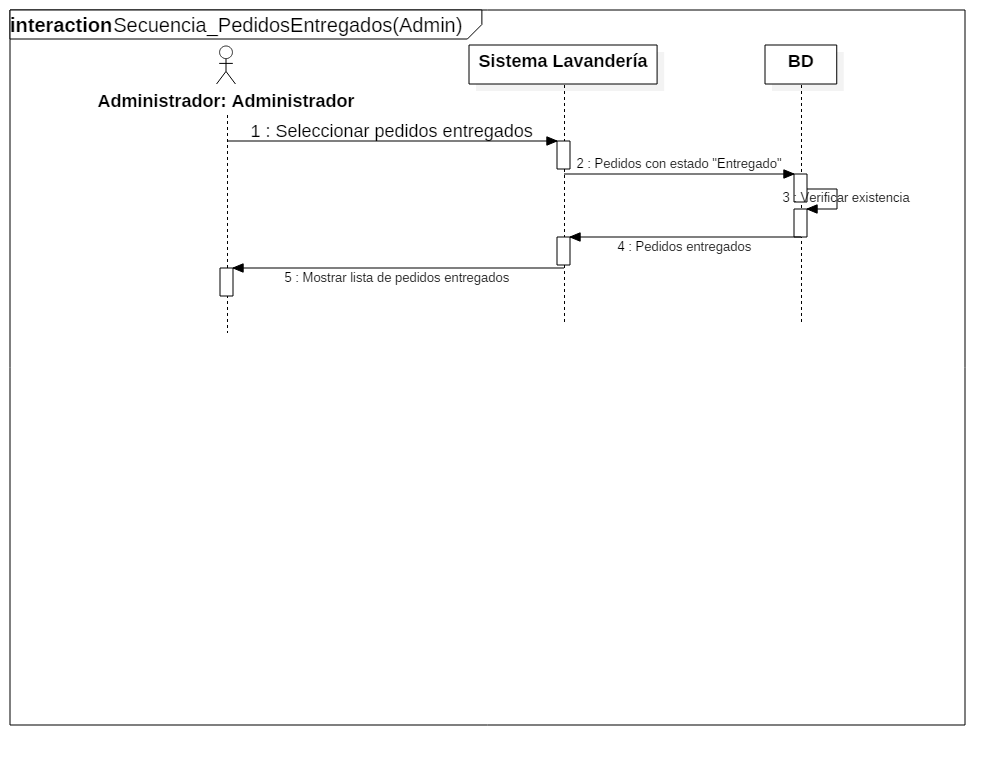
\includegraphics[width=10cm]{./imagenes/diagramas/Secuencia_PedidosEntregados(Admin).png}
\end{center}
\caption{Diagrama de Secuencia: Pedidos entregados -Admin}
\end{figure}


\begin{figure}[htb]
\begin{center}
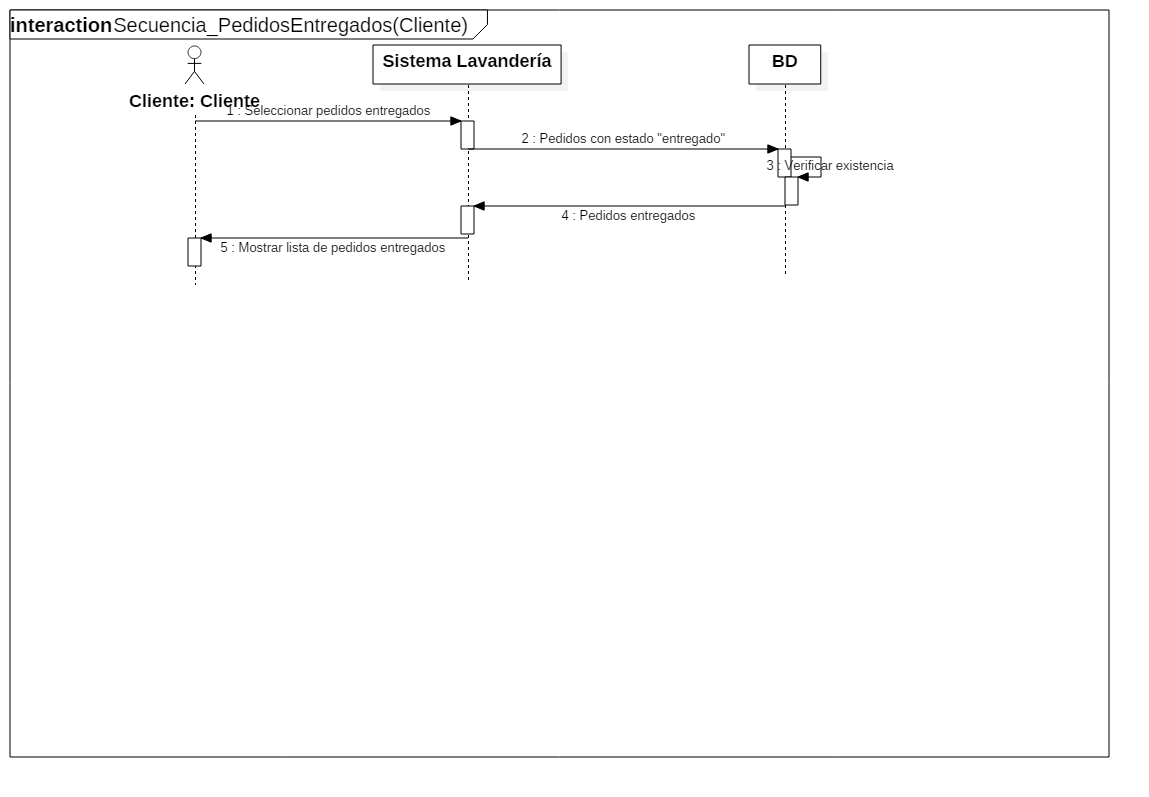
\includegraphics[width=10cm]{./imagenes/diagramas/Secuencia_PedidosEntregados(Cliente).png}
\end{center}
\caption{Diagrama de Secuencia: Pedidos entregados -Cliente}
\end{figure}


\begin{figure}[htb]
\begin{center}
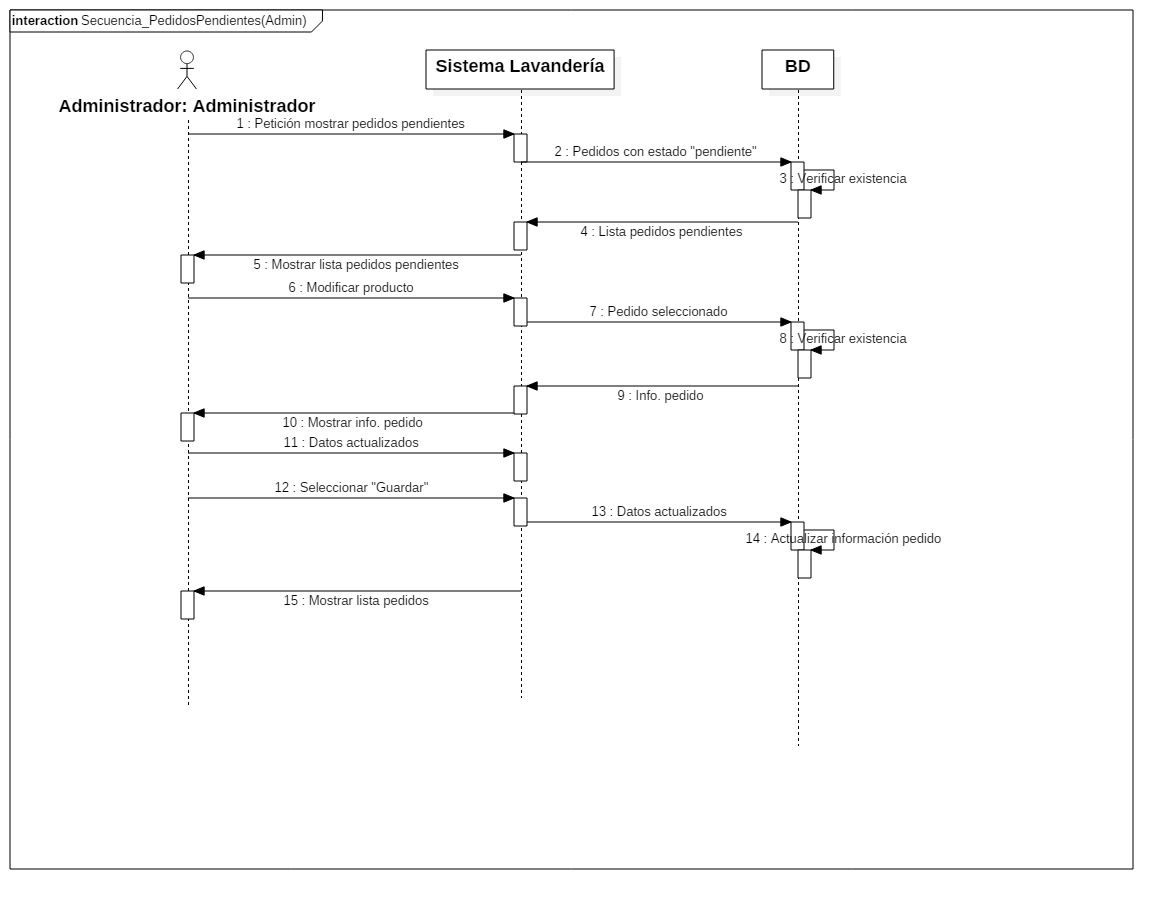
\includegraphics[width=10cm]{./imagenes/diagramas/Secuencia_PedidosPendientes(Admin).png}
\end{center}
\caption{Diagrama de Secuencia: Pedidos Pendientes -Admin }
\end{figure}


\begin{figure}[htb]
\begin{center}
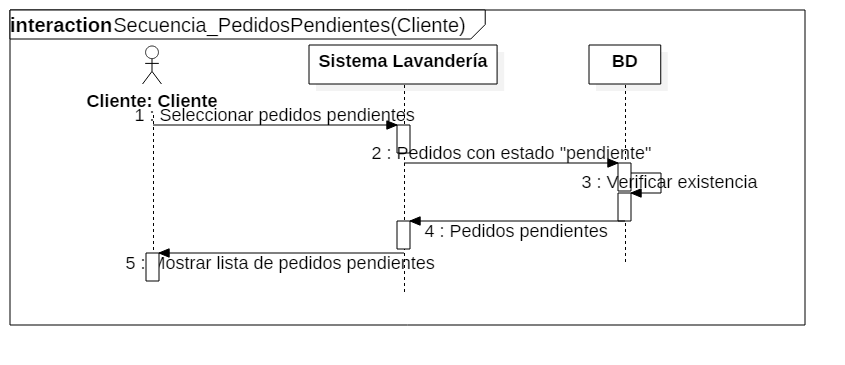
\includegraphics[width=10cm]{./imagenes/diagramas/Secuencia_PedidosPendientes(Cliente).png}
\end{center}
\caption{Diagrama de Secuencia: Pedidos Pendientes -Cliente}
\end{figure}



\begin{figure}[htb]
\begin{center}
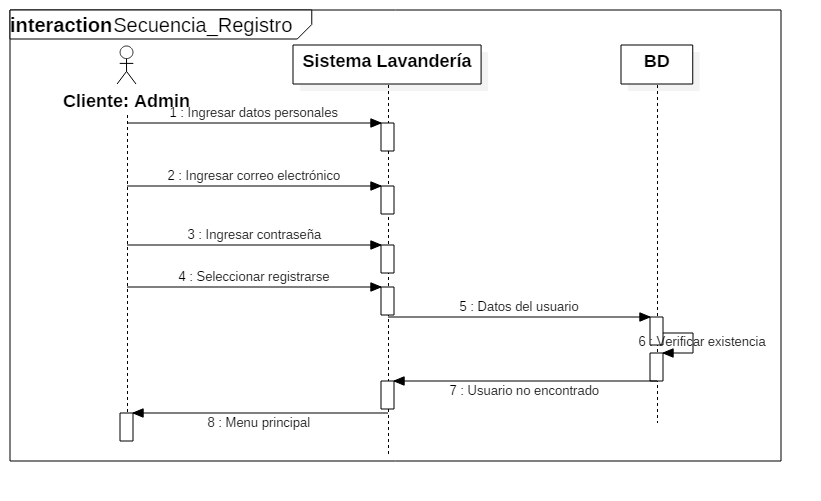
\includegraphics[width=10cm]{./imagenes/diagramas/Secuencia_Registro.png}
\end{center}
\caption{Diagrama de Secuencia: Registro}
\end{figure}




\newpage




\subsubsection{Diagrama de componentes y distribucion}


\begin{figure}[h]
\begin{center}
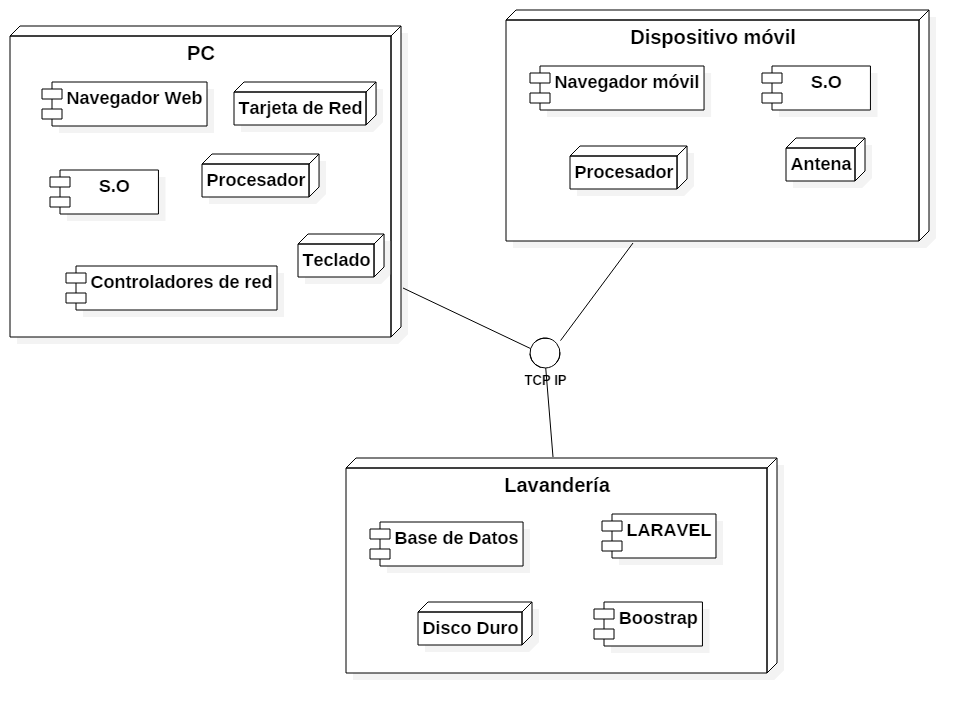
\includegraphics[width=20cm]{./imagenes/diagramas/Com-Dis_Lavanderia.png}
\end{center}
\caption{Diagrama de Componentes}
\end{figure}




